\documentclass[11pt,a4paper]{article}
\usepackage[margin=0.8in]{geometry}
\usepackage[T1]{fontenc}
\usepackage[utf8]{inputenc}
\usepackage{lmodern}
\usepackage{amsmath,amssymb}
\usepackage{graphicx}
\usepackage{caption}
\usepackage{booktabs}
\usepackage{longtable}
\usepackage{tabularx}
\usepackage{enumitem}
\usepackage{hyperref}
\usepackage[table]{xcolor}
\usepackage{float}
\usepackage{pdflscape}
 
\definecolor{aybu_blue}{RGB}{31, 73, 125}
\hypersetup{colorlinks=true, linkcolor=aybu_blue, urlcolor=blue}
\graphicspath{{./diagrams_aybustore/}}
 
% --- Colour palette used by the new tables and the Gantt chart (sections 3.4 / 3.5)
\definecolor{aybuHeader}{RGB}{46, 117, 182}
\definecolor{aybuAlt}{RGB}{242, 242, 242}
\definecolor{aybuBlock}{RGB}{221, 235, 247}
\definecolor{ganttActive}{RGB}{46, 117, 182}
\definecolor{ganttBuffer}{RGB}{189, 215, 238}
\definecolor{ganttSprint}{RGB}{255, 242, 204}
\definecolor{ganttMile}{RGB}{244, 176, 132}
\definecolor{riskMed}{RGB}{255, 235, 156}
\definecolor{riskHigh}{RGB}{248, 203, 173}
 
% --- Helper macros for the Gantt chart cells
\providecommand{\GA}{\cellcolor{ganttActive}}
\providecommand{\GB}{\cellcolor{ganttBuffer}}
 
% Prevent headers from being separated from text
\widowpenalty=10000
\clubpenalty=10000
\interlinepenalty=500
\raggedbottom
 
\title{\LARGE \textbf{AYBUStore: Intelligent Campus E-Commerce Ecosystem}\\[0.5em] \large \textbf{CENG306 Term Project Final Proposal}}
\author{\textbf{Muhammed Yıldız (myz21)}, Utkan Dindaroğlu, Ahmet Selim Yılmaz, \\ Seyfullah Gülyazı, Süleyman Fatih Sert}
\date{Spring 2025--2026}
 
\begin{document}
 
\maketitle
 
\section{Abstract}
AYBUStore is a university-centered, hyper-local closed-loop digital commerce project designed to eliminate unequal access created by Ankara Yıldırım Beyazıt University's multi-campus structure (Esenboğa, Etlik, Bilkent, and Çubuk). The platform transforms a single-point physical service model into a continuous and location-independent digital ecosystem for intra-university use, integrating a modern front-end, scalable back-end, and rule-based automated support modules in one end-to-end architecture. Within a 3-month pilot, the project targets measurable outcomes aligned with institutional needs: at least a 30\% increase in cross-campus accessibility, at least 40\% improvement in Time to Interactive (TTI) from a baseline of approximately 3.5 seconds to below 1.5 seconds, and significant operational gains through a 60\% reduction in first support response time and at least 45\% reduction in average issue-resolution time. Evaluation is designed on log-based performance indicators collected from at least 300 active SIS-verified students, with comparative statistical testing against baseline system data.
 
\section{Problem Definition \& Motivation}
AYBU currently operates with a single-point physical market model, while students are distributed across four campuses. This creates unequal access to routine needs, avoidable travel/time costs, and fragmented service continuity for students outside the main store location.
 
The impact is both practical and academic: service inequality reduces day-to-day student welfare, manual and location-bound workflows limit institutional operational efficiency, and the university context remains underrepresented in existing e-commerce research. Current alternatives (physical-only supply and static portal-style access) are insufficient because they do not provide continuous cross-campus availability, measurable responsiveness targets (TTI), or integrated support automation for fast issue handling. AYBUStore is motivated by this gap and proposes a campus-specific digital commerce layer designed for equitable access and verifiable performance.
 
\section{Literature Review}
We reviewed 12 peer-reviewed studies and analyzed each one against AYBUStore's target context.
\begin{itemize}
    \item \textbf{Gong \& Yi (2018)} validates service quality as a driver of satisfaction and loyalty, but it is not specific to campus logistics or distributed access conditions.
    \item \textbf{Alsheyadi \& Albalushi (2020)} examines student service quality and collaboration effects, yet does not model digital supply flows for physical student needs.
    \item \textbf{Brdesee \& Alsaggaf (2022)} improves university e-services through decision and process redesign, but the scope is advising/registration rather than campus commerce operations.
    \item \textbf{Alenezi \& Akour (2023)} provides a digital transformation blueprint for higher education, but remains strategic and does not define an end-to-end operational architecture with measurable commerce KPIs.
    \item \textbf{Urquhart et al. (2022)} identifies last-mile capacity constraints in online grocery systems, but in a national retail setting rather than a closed university ecosystem.
    \item \textbf{Suryawanshi et al. (2021)} presents resilient hyperlocal grocery planning under uncertainty, yet does not address campus equity or student-centered service continuity.
    \item \textbf{Liu et al. (2021)} optimizes sustainable urban e-grocery distribution networks, but focuses on routing and cost objectives instead of institutional access fairness.
    \item \textbf{Melkonyan et al. (2020)} compares sustainable last-mile strategies in local food networks, but does not integrate authentication-bound user communities and support workflows.
    \item \textbf{Netravali et al. (2018)} introduces robust TTI measurement (Ready Index), but does not connect performance metrics to equitable service delivery outcomes.
    \item \textbf{Jahromi et al. (2020)} extends web QoE evaluation beyond first-page load, but not in university marketplace environments with operational constraints.
    \item \textbf{Güldal \& Dinçer (2025)} shows that rule-based chatbots are acceptable in higher education, yet does not embed them into issue-resolution pipelines for commerce processes.
    \item \textbf{Dinh \& Tran (2023)} demonstrates a hybrid university-information chatbot, but not transaction-aware support automation linked to order and ticket lifecycles.
\end{itemize}
 
The common gap is clear: prior work treats service quality, campus digitalization, hyperlocal logistics, web performance, and chatbot support as separate tracks. AYBUStore fills this gap by combining them in a single closed-loop intra-university model with measurable pilot targets: at least 30\% cross-campus access improvement, TTI reduction from approximately 3.5s to below 1.5s, and faster support operations through rule-based automation.
 
\textit{Full bibliographic details for all reviewed studies are provided in the References section.}
 
\newpage
% ============================================================
% SECTION 4: OBJECTIVES & SCOPE
% ============================================================
\section{Objectives \& Scope}
\label{sec:objectives-scope}
 
\subsection{Project Objectives}
AYBUStore is defined in this report as a university-centered,
closed-loop digital commerce ecosystem for AYBU campuses. In alignment
with the Abstract, Problem Definition, and UML sections, the project
focuses on equitable cross-campus access, OTP-based secure entry,
AI-assisted discovery/support, and campus-aware order operations.
The five measurable objectives below define success criteria for the
3-month pilot evaluation.
 
\renewcommand{\arraystretch}{1.25}
\begin{table}[H]
\centering
\small
\begin{tabular}{|p{0.06\textwidth}|p{0.22\textwidth}|p{0.40\textwidth}|p{0.18\textwidth}|}
\hline
\rowcolor{aybuHeader}
\textcolor{white}{\textbf{ID}} &
\textcolor{white}{\textbf{Objective}} &
\textcolor{white}{\textbf{Description}} &
\textcolor{white}{\textbf{Success Metric}} \\ \hline
 
OBJ-1 & Increase cross-campus service access equity &
Improve effective access for students located outside the main store
campus by ensuring that ordering and support are continuously available
through a single digital channel across Esenboğa, Etlik, Bilkent, and
Çubuk campuses. &
$\geq 30\%$ increase in peripheral-campus active utilization versus
baseline; at least 300 active SIS-verified users in pilot. \\ \hline
 
OBJ-2 & Ensure secure access control &
Implement and operate OTP-based authentication and verification
controls so that only authorized university users can access protected
flows and user-specific order/support data. &
100\% of registered users authenticate through OTP flow; zero critical
auth bypass findings in release checklist. \\ \hline
 
OBJ-3 & Improve platform responsiveness (TTI) &
Optimize storefront rendering and interaction readiness to reduce
latency-related abandonment and support consistent use under typical
campus network conditions. &
At least 40\% improvement versus baseline (approx.\ 3.5s), with average
TTI $< 1.5$s on pilot measurements. \\ \hline
 
OBJ-4 & Improve support operation efficiency &
Integrate rule-based AI assistance and ticket routing into the order
lifecycle so common issues are answered faster and escalations are
tracked with reduced manual overhead. &
At least 60\% reduction in first response time and at least 45\%
reduction in average issue-resolution time versus baseline. \\ \hline
 
OBJ-5 & Preserve operational reliability in pilot &
Maintain stable order, inventory, and notification operations while
handling pilot traffic and preserving transaction integrity. &
99.9\% service uptime during pilot window, 0\% transaction-level data
loss, and stable operation at defined peak test load. \\ \hline
\end{tabular}
\caption{AYBUStore measurable project objectives.}
\label{tab:objectives}
\end{table}
 
\subsection{In-Scope Capabilities}
The following items are explicitly within scope for AYBUStore and are
consistent with the use case, activity, and sequence diagrams included
in this report:
\begin{itemize}[leftmargin=*]
    \item \textbf{Campus-focused digital storefront} --- product
    catalogue browsing, keyword-based search, and customizable
    merchandise flows for intra-university use.
    \item \textbf{Secure OTP authentication} --- OTP-based registration
    and login verification for protected user/order actions.
    \item \textbf{Order lifecycle and campus-aware operations} ---
    cart, checkout, order placement, campus route determination, and
    status progression with operational visibility.
    \item \textbf{Real-time tracking and notifications} --- user-facing
    tracking updates and event-driven notifications tied to order state
    changes.
    \item \textbf{AI-assisted interaction layer} --- rule-based AI
    assistance for product discovery and first-level support handling.
    \item \textbf{Admin/CMS operations} --- inventory and catalogue
    management, order/rule administration, and operational monitoring
    features needed by campus operations.
    \item \textbf{Pilot evaluation instrumentation} --- collection of
    TTI, access-utilization, and support-resolution indicators required
    for objective-based evaluation.
\end{itemize}
 
\subsection{Out-of-Scope Items}
To keep the project aligned with the current pilot and semester
constraints, the items below are explicitly out of scope in this phase:
\begin{itemize}[leftmargin=*]
    \item \textbf{Third-party payment gateway production integration}
    (Stripe/iyzico live operations); payment is treated as simulated in
    this phase.
    \item \textbf{Off-campus or city-wide delivery operations}; scope is
    limited to AYBU campus ecosystem and intra-university routing.
    \item \textbf{Integration with external/non-project academic
    platforms} beyond required identity and project-specific data flows.
    \item \textbf{Advanced predictive AI/ML modules} (e.g., deep
    personalization, forecasting, vision-based recommendation) beyond
    the defined rule-based assistant layer.
    \item \textbf{Enterprise ERP/finance/warehouse integration} and
    full institutional procurement automation.
    \item \textbf{Native desktop client products} and broad public
    marketplace expansion.
\end{itemize}
 
% ============================================================
% SECTION 5: METHODOLOGY & DEVELOPMENT PLAN
% ============================================================
\section{Methodology \& Development Plan}
\label{sec:methodology}
 
\subsection{Software Development Lifecycle}
The AYBUStore project follows the \textbf{Agile / Scrum} software
development lifecycle. The team consists of five developers working
over a 14--15 week academic semester, with weekly checkpoints,
evolving requirements (especially in the UI/UX and payment-integration
areas), and a deliverable-driven academic calendar --- conditions that
align strongly with iterative, incremental delivery.
 
\subsubsection*{Justification of Process Model Choice}
Three candidate models were considered: \emph{Waterfall},
\emph{Spiral}, and \emph{Agile/Scrum}. Each was evaluated against the
project's defining characteristics.
 
\begin{table}[H]
\centering
\small
\begin{tabular}{|p{0.18\textwidth}|p{0.38\textwidth}|p{0.34\textwidth}|}
\hline
\rowcolor{aybuHeader}
\textcolor{white}{\textbf{Model}} &
\textcolor{white}{\textbf{Strengths for this project}} &
\textcolor{white}{\textbf{Weaknesses for this project}} \\ \hline
 
Waterfall & Clear documentation; well-suited to fully understood
requirements; easy progress tracking. & UI/UX requirements are
expected to evolve through stakeholder feedback; campus-routing and
support-automation flows carry discovery risk that Waterfall handles
poorly. \\ \hline
 
Spiral & Strong emphasis on risk analysis at each cycle; useful for
high-risk financial systems. & Overhead of full risk-driven cycles is
excessive for a 14-week academic project; cost of repeated full-scale
risk analysis outweighs benefit. \\ \hline
 
\textbf{Agile / Scrum} \emph{(selected)} & Two-week sprints align with
academic checkpoints; iterative delivery accommodates UI/UX changes;
daily stand-ups suit a 5-person collocated team; backlog supports
MoSCoW prioritization of must-have vs. nice-to-have features. &
Requires self-discipline in ceremony attendance; documentation must
be produced alongside iterations rather than upfront --- mitigated by
treating SRS, design, and test plan as evolving artefacts updated
each sprint. \\ \hline
\end{tabular}
\caption{Comparison of candidate process models for AYBUStore.}
\label{tab:process-models}
\end{table}
 
The team will run \textbf{seven 2-week sprints}. Each sprint begins
with sprint planning (selecting items from the product backlog), is
followed by daily 15-minute stand-ups, and ends with a sprint review
(demo to the team's academic advisor) and a sprint retrospective.
Roles are assigned as follows: one \emph{Product Owner} (manages
backlog and stakeholder communication), one \emph{Scrum Master}
(facilitates ceremonies and removes blockers), and three
\emph{Developers}. All five members contribute to coding tasks
regardless of role.
 
\subsection{Work Breakdown Structure (WBS)}
\label{subsec:wbs}
The work to be performed has been decomposed into five top-level work
packages, each containing several deliverable-oriented activities.
The numbering follows the standard hierarchical WBS convention.
 
\renewcommand{\arraystretch}{1.2}
\begin{table}[H]
\centering
\small
\begin{tabular}{|p{0.07\textwidth}|p{0.27\textwidth}|p{0.55\textwidth}|}
\hline
\rowcolor{aybuHeader}
\textcolor{white}{\textbf{WBS ID}} &
\textcolor{white}{\textbf{Work Package}} &
\textcolor{white}{\textbf{Description / Deliverables}} \\ \hline
 
\rowcolor{aybuBlock}
\textbf{1.0} & \textbf{Project Initiation \& Planning} &
Vision and scope definition; team-role assignment; technology stack
confirmation; communication plan. \\ \hline
1.1 & Stakeholder \& vision workshop & Half-day workshop with academic
advisor; output: project vision statement. \\ \hline
1.2 & Tooling and repository setup & GitHub repository, Firebase
project, Jira/Trello board, CI workflow skeleton. \\ \hline
 
\rowcolor{aybuBlock}
\textbf{2.0} & \textbf{Requirements Engineering} & Full SRS document
including functional and non-functional requirements, use cases, UML
diagrams. \\ \hline
2.1 & Functional requirements \& use cases & Catalogue, cart/checkout,
accounts, inventory, tracking/support use cases. \\ \hline
2.2 & Non-functional requirements & Performance, security, usability,
accessibility, maintainability targets. \\ \hline
2.3 & UML modelling & Use case, activity, sequence, and analysis
object model diagrams. \\ \hline
 
\rowcolor{aybuBlock}
\textbf{3.0} & \textbf{System Design} & Architectural and detailed
design artefacts. \\ \hline
3.1 & System architecture & Client--server architecture with
responsive web client + Firebase; module decomposition. \\ \hline
3.2 & Data model design & Firestore collection schema for users,
products, categories, orders, support tickets. \\ \hline
3.3 & UI/UX design & Wireframes, high-fidelity mock-ups (Figma),
design system, accessibility check. \\ \hline
3.4 & API \& integration design & Cloud Function endpoints,
OTP verification and notification integration contract. \\ \hline
 
\rowcolor{aybuBlock}
\textbf{4.0} & \textbf{Implementation (Sprints)} & Iterative
development across 7 two-week sprints (documentation-only deliverable
means coding produces reference implementations for design
validation). \\ \hline
4.1 & Authentication module & Sign-up, login, password reset, AYBU
identity flag (Sprint~1--2). \\ \hline
4.2 & Catalogue \& search module & Product list, detail page,
filtering, keyword search (Sprint~2--3). \\ \hline
4.3 & Cart \& checkout module & Cart persistence, address book,
simulated payment confirmation flow (Sprint~3--4). \\ \hline
4.4 & Admin \& inventory module & Product/inventory CRUD, low-stock
alerts, order management (Sprint~4--5). \\ \hline
4.5 & Tracking \& support module & Real-time tracking updates,
rule-based AI support, and ticket routing (Sprint~5--6). \\ \hline
 
\rowcolor{aybuBlock}
\textbf{5.0} & \textbf{Verification, Validation \& Closure} & Quality
assurance and final delivery. \\ \hline
5.1 & Unit \& integration testing & Jest unit tests for business
logic; integration tests for OTP and order-tracking flow. \\ \hline
5.2 & System \& acceptance testing & End-to-end test scenarios derived
from use cases; UAT with advisor. \\ \hline
5.3 & Final documentation \& defence & Final SRS, design document,
test report, user manual; project defence presentation. \\ \hline
\end{tabular}
\caption{Hierarchical Work Breakdown Structure for AYBUStore.}
\label{tab:wbs}
\end{table}
 
\subsection{Gantt Chart}
\label{subsec:gantt}
The project is scheduled over 15 weeks, organized as one preparation
week followed by seven 2-week Scrum sprints. The Gantt chart below
tracks each WBS work package against the project timeline; filled
cells indicate active work, light cells indicate review/buffer
activity, and the bottom row marks milestone deliverables.
 
\renewcommand{\arraystretch}{1.15}
\begin{table}[H]
\centering
\scriptsize
\setlength{\tabcolsep}{2pt}
\begin{tabular}{|p{2.8cm}|*{15}{c|}}
\hline
\rowcolor{aybuHeader}
\textcolor{white}{\textbf{Activity / Week}} &
\textcolor{white}{\textbf{W1}} & \textcolor{white}{\textbf{W2}} &
\textcolor{white}{\textbf{W3}} & \textcolor{white}{\textbf{W4}} &
\textcolor{white}{\textbf{W5}} & \textcolor{white}{\textbf{W6}} &
\textcolor{white}{\textbf{W7}} & \textcolor{white}{\textbf{W8}} &
\textcolor{white}{\textbf{W9}} & \textcolor{white}{\textbf{W10}} &
\textcolor{white}{\textbf{W11}} & \textcolor{white}{\textbf{W12}} &
\textcolor{white}{\textbf{W13}} & \textcolor{white}{\textbf{W14}} &
\textcolor{white}{\textbf{W15}} \\ \hline
 
\rowcolor{ganttSprint}
\textbf{Sprint structure} & Prep & \multicolumn{2}{c|}{Sprint 1} &
\multicolumn{2}{c|}{Sprint 2} & \multicolumn{2}{c|}{Sprint 3} &
\multicolumn{2}{c|}{Sprint 4} & \multicolumn{2}{c|}{Sprint 5} &
\multicolumn{2}{c|}{Sprint 6} & \multicolumn{2}{c|}{Sprint 7} \\ \hline
 
1.0 Initiation \& Planning & \GA & \GA & & & & & & & & & & & & & \\ \hline
2.0 Requirements Eng. & \GA & \GA & \GA & \GB & \GB & & & & & & & & & & \\ \hline
3.0 System Design & & \GA & \GA & \GA & \GA & \GB & \GB & & & & & & & & \\ \hline
4.1 Authentication module & & \GA & \GA & \GA & \GA & & & & & & & & & & \\ \hline
4.2 Catalogue \& search & & & & \GA & \GA & \GA & \GA & & & & & & & & \\ \hline
4.3 Cart \& checkout & & & & & & \GA & \GA & \GA & \GA & & & & & & \\ \hline
4.4 Admin \& inventory & & & & & & & & \GA & \GA & \GA & \GA & & & & \\ \hline
4.5 Tracking \& support & & & & & & & & & & \GA & \GA & \GA & \GA & & \\ \hline
5.1 Unit \& integration test & & & & \GB & \GB & \GB & \GB & \GB & \GB & \GB & \GA & \GA & \GA & & \\ \hline
5.2 System \& acceptance test & & & & & & & & & & & & & \GA & \GA & \\ \hline
5.3 Final docs \& defence & & & & & & & & & & & & & & \GA & \GA \\ \hline
 
\rowcolor{ganttMile}
\textbf{Milestones} & & & SRS & & & & Design & & & & MVP & & Test & & Final \\ \hline
\end{tabular}
\caption{15-week Gantt chart for AYBUStore. Dark blue = active work,
light blue = review/buffer, orange = milestone deliverable.}
\label{tab:gantt}
\end{table}
 
\noindent
\textbf{Key milestones:} SRS baseline (end of W3), design document
baseline (end of W7), feature-complete MVP for documentation
(end of W11), full test report (end of W13), and final delivery with
defence (end of W15).
 
\subsection{Effort and Cost Estimation}
\label{subsec:effort-cost}
Effort and cost have been estimated using the \textbf{COCOMO}
(Constructive Cost Model) Basic model, which derives effort from
estimated source-lines-of-code (KLOC). COCOMO was preferred over
Function Point Analysis because the team has higher confidence in
code-size estimation than in transaction-counting for a
Firebase-backed BaaS architecture.
 
\subsubsection*{Size Estimation}
Lines of code have been estimated module by module based on
comparable open-source university-commerce references built on
web front-end + Firebase backends.
The estimate excludes auto-generated configuration files and
third-party library code.
 
\begin{table}[H]
\centering
\small
\begin{tabular}{|p{0.30\textwidth}|p{0.45\textwidth}|p{0.16\textwidth}|}
\hline
\rowcolor{aybuHeader}
\textcolor{white}{\textbf{Module}} &
\textcolor{white}{\textbf{Notes}} &
\textcolor{white}{\textbf{Estimated LOC}} \\ \hline
 
Authentication \& user profile & Firebase Auth wiring, registration
form, AYBU verification flag, profile page. & 900 \\ \hline
Catalogue \& search & Product list, detail screen, filters, keyword
search, pagination. & 1{,}500 \\ \hline
Cart \& checkout & Cart state, address book, simulated payment
confirmation flow, order confirmation. & 1{,}200 \\ \hline
Admin \& inventory panel & Web admin UI, CRUD for products /
categories, inventory dashboard, order management. & 1{,}400 \\ \hline
Tracking \& support & Tracking status events, AI-assisted support, and
ticket lifecycle handling. & 700 \\ \hline
Cloud Functions (backend logic) & OTP/session checks, stock deduction,
order state machine, routing and notifications. & 800 \\ \hline
\textbf{Total} & \textbf{Sum across all modules.} &
\textbf{6{,}500 LOC} \\ \hline
\end{tabular}
\caption{Module-by-module LOC estimate for AYBUStore.}
\label{tab:kloc}
\end{table}
 
\subsubsection*{COCOMO Basic Calculation}
AYBUStore is classified as an \emph{Organic} project: a small,
experienced team (5 developers, all senior undergraduates) developing
a relatively well-understood application (CRUD-centric e-commerce) in
a familiar environment. The Basic COCOMO coefficients for an Organic
project are $a = 2.4$, $b = 1.05$ for effort and $c = 2.5$, $d = 0.38$
for schedule.
 
\begin{table}[H]
\centering
\small
\begin{tabular}{|p{0.30\textwidth}|p{0.45\textwidth}|p{0.16\textwidth}|}
\hline
\rowcolor{aybuHeader}
\textcolor{white}{\textbf{Metric}} &
\textcolor{white}{\textbf{Formula}} &
\textcolor{white}{\textbf{Result}} \\ \hline
 
Estimated size & From the module-by-module estimate above. & 6.5 KLOC \\ \hline
Effort (person-months) & $E = 2.4 \times (6.5)^{1.05} = 2.4 \times 7.16$ & $\approx$ 17.2 PM \\ \hline
Development time (months) & $T = 2.5 \times (17.2)^{0.38} = 2.5 \times 2.95$ & $\approx$ 7.4 months \\ \hline
Required team size & $N = E / T = 17.2 / 7.4$ & $\approx$ 2.3 people \\ \hline
Productivity & $P = $ KLOC$ / E = 6{,}500 / 17.2$ & $\approx$ 378 LOC/PM \\ \hline
\end{tabular}
\caption{Basic COCOMO calculation for AYBUStore (Organic mode).}
\label{tab:cocomo}
\end{table}
 
\noindent
\textbf{Interpretation.} Basic COCOMO predicts approximately
17.2 person-months and a 7.4-month nominal schedule for a full build.
The project team has 5 developers and a 3.5-month academic calendar
($\approx$ 15 weeks), yielding available effort of about 17.5 PM.
Therefore, the pilot remains feasible only with strict scope control:
reference-level implementation depth, simulated payment flow,
prioritized must-have features, and documentation-first acceptance.
 
\subsubsection*{Cost Estimation}
For an academic project no labour cost is paid out; nevertheless a
notional cost is computed to indicate the project's commercial value,
using a junior-developer rate of \$1{,}500 per person-month --- a
representative regional figure for Turkey for an entry-level
full-stack developer.
 
\begin{table}[H]
\centering
\small
\begin{tabular}{|p{0.36\textwidth}|p{0.40\textwidth}|p{0.16\textwidth}|}
\hline
\rowcolor{aybuHeader}
\textcolor{white}{\textbf{Cost component}} &
\textcolor{white}{\textbf{Calculation}} &
\textcolor{white}{\textbf{Amount}} \\ \hline
 
Notional labour & $17.2$~PM $\times$ \$1{,}500 & $\approx$ \$25{,}800 \\ \hline
Infrastructure (Firebase Spark/Blaze, dev only) & Mostly free-tier;
minor overages during testing. & $\approx$ \$100 \\ \hline
Payment simulation tooling & Simulated checkout only; no live
transaction processing in this phase. & \$0 \\ \hline
Tooling (Figma, GitHub, IDE) & Free or academic-license tiers. & \$0 \\ \hline
\textbf{Total estimated project cost} & \textbf{Sum of all components.} & \boldmath{$\approx$ \$25{,}900} \\ \hline
\end{tabular}
\caption{Notional cost estimate for AYBUStore.}
\label{tab:cost}
\end{table}
 
\subsection{Risk Management}
\label{subsec:risk}
The register below records the principal risks identified at project
inception. Each risk is rated on \emph{probability} (Low / Medium /
High), \emph{impact} (Low / Medium / High), and assigned an
\emph{exposure} level computed as Probability $\times$ Impact (where
Low = 1, Medium = 2, High = 3, so exposure values of 1--2 are Low,
3--4 are Medium, and 6--9 are High). The risk register will be
reviewed at the start of every sprint as part of sprint planning.
 
\renewcommand{\arraystretch}{1.2}
\begin{table}[H]
\centering
\footnotesize
\begin{tabular}{|p{0.04\textwidth}|p{0.22\textwidth}|p{0.05\textwidth}|p{0.05\textwidth}|p{0.06\textwidth}|p{0.28\textwidth}|p{0.05\textwidth}|}
\hline
\rowcolor{aybuHeader}
\textcolor{white}{\textbf{ID}} &
\textcolor{white}{\textbf{Risk Description}} &
\textcolor{white}{\textbf{Prob.}} &
\textcolor{white}{\textbf{Imp.}} &
\textcolor{white}{\textbf{Expos.}} &
\textcolor{white}{\textbf{Mitigation Strategy}} &
\textcolor{white}{\textbf{Owner}} \\ \hline
 
R1 & Campus-routing and notification integration delays ---
event-driven tracking and campus route logic may require more iteration
than estimated. & High & High &
\cellcolor{riskHigh}\textbf{High} & Start integration spike in
Sprint~1; define minimal route/notification contract early; implement a
feature flag for fallback status updates; allocate buffer in
Sprints~3--4. & PO \\ \hline
 
R2 & Scope creep --- stakeholders request additional features
(loyalty, multi-vendor, advanced search) mid-project. & High & Med &
\cellcolor{riskMed}\textbf{Med} & Maintain a strict MoSCoW-prioritized
backlog; require any new request to displace an existing backlog item
of equal effort; product owner is the single point of acceptance. &
PO \\ \hline
 
R3 & Team-member unavailability --- illness, exam load, or course
conflicts reduce effective capacity below the planned 5 developers. &
Med & High & \cellcolor{riskHigh}\textbf{High} & Cross-pair on critical
modules so no module has a single owner; maintain up-to-date task
documentation; reserve 15\% buffer in every sprint; reassign tasks
during stand-ups when needed. & SM \\ \hline
 
R4 & Security and data-protection breaches --- leaked credentials,
exposed PII, or insecure direct object references in admin endpoints.
& Med & High & \cellcolor{riskHigh}\textbf{High} & Enforce Firebase
Security Rules with deny-by-default; mandatory code review for all
auth and admin code paths; secrets stored only in environment
variables; OWASP ASVS Level~1 checklist run before final delivery. &
Dev \\ \hline
 
R5 & Performance bottlenecks under load --- slow Firestore queries,
unindexed search, or unoptimized images cause UX targets to be missed.
& Med & Med & \cellcolor{riskMed}\textbf{Med} & Define indexed query
patterns at design time; introduce pagination on all list views;
lazy-load images with a CDN; run a load test in Sprint~6 to validate
the 500-concurrent-user target. & Dev \\ \hline
 
R6 & Inadequate testing coverage --- limited time for QA in the final
sprint produces undetected defects. & Med & Med &
\cellcolor{riskMed}\textbf{Med} & Adopt test-as-you-build: every PR
includes unit tests; integration tests for OTP, routing, and order
tracking flow written by W8; final sprint reserved for system and
acceptance testing only. & Dev \\ \hline
 
R7 & Third-party service outages --- Firebase or notification service
downtime blocks development or testing. & Low & High &
\cellcolor{riskMed}\textbf{Med} & Maintain local Firebase emulator
suite for offline development; keep mock notification stubs available;
subscribe to service status notifications. & Dev \\ \hline
 
R8 & Documentation drift --- code evolves through sprints but the SRS
/ design document is not kept current, jeopardizing the final
documentation-only deliverable. & Med & High &
\cellcolor{riskHigh}\textbf{High} & Treat documentation updates as a
Definition-of-Done criterion for every story; assign a rotating
``doc owner'' per sprint; reserve W14--W15 entirely for final document
polish. & PO \\ \hline
\end{tabular}
\caption{AYBUStore risk register
(PO = Product Owner, SM = Scrum Master, Dev = Developer team).}
\label{tab:risks}
\end{table}
 
\noindent
Risks will be re-rated at every sprint retrospective. Any risk that
materializes will be moved into an issues register, and any risk
whose exposure rises to High will trigger an out-of-band review with
the academic advisor.
 
% ============================================================
% SECTION 6: REQUIREMENTS SPECIFICATION (SRS)
% ============================================================
\section{Requirements Specification (SRS)}
\label{sec:srs}
This section presents the Software Requirements Specification for AYBUStore, organized into functional requirements, non-functional requirements with measurable acceptance criteria, user stories, and the use case model.
 
\subsection{Functional Requirements}
\renewcommand{\arraystretch}{1.2}
\begin{longtable}{|p{0.08\textwidth}|p{0.25\textwidth}|p{0.60\textwidth}|}
\hline
\rowcolor{aybuHeader}
\textcolor{white}{\textbf{ID}} &
\textcolor{white}{\textbf{Requirement}} &
\textcolor{white}{\textbf{Description}} \\ \hline \endhead
FR-01 & SIS-Based Registration & The system shall allow students to register using their AYBU SIS credentials and verify identity through a 6-digit OTP delivered to their institutional email. \\ \hline
FR-02 & Secure Authentication & The system shall authenticate returning users via email/password combined with session tokens managed by Firebase Authentication. \\ \hline
FR-03 & Product Catalog Browsing & The system shall display the full product catalog with category filters, price range, size, and campus-availability filters. \\ \hline
FR-04 & AI-Assisted Search & The system shall accept natural-language queries (e.g., ``white sweatshirt under 500 TL'') and return ranked product matches via the intent-analysis module. \\ \hline
FR-05 & Cart Management & The system shall allow authenticated users to add, update quantity, remove, and persist cart items across sessions and devices. \\ \hline
FR-06 & Order Placement \& Simulated Payment & The system shall accept order submissions with a simulated payment confirmation and generate a unique order ID with timestamp. \\ \hline
FR-07 & Campus-Specific Logistics Routing & The system shall route each order to the nearest fulfillment node among the four AYBU campuses (Esenboğa, Etlik, Bilkent, Çubuk) based on user selection. \\ \hline
FR-08 & Real-Time Order Tracking & The system shall display order status transitions (Placed $\rightarrow$ Prepared $\rightarrow$ In-Transit $\rightarrow$ Delivered) updated in real time via Firestore listeners. \\ \hline
FR-09 & Admin Stock Management & The system shall provide an Admin CMS where authorized staff can create, update, and deactivate products and adjust stock levels. \\ \hline
FR-10 & Notification Dispatch & The system shall send email and in-app notifications on order confirmation, status changes, and support-ticket updates. \\ \hline
FR-11 & Support Ticketing with Rule-Based Bot & The system shall let users open support tickets; a rule-based chatbot shall attempt first-line resolution before human escalation. \\ \hline
FR-12 & Audit Logging & The system shall record authentication events, admin actions, and order state changes in an immutable audit log for traceability. \\ \hline
\caption{AYBUStore functional requirements.} \label{tab:fr} \\
\end{longtable}
 
\subsection{Non-Functional Requirements}
\begin{longtable}{|p{0.08\textwidth}|p{0.22\textwidth}|p{0.63\textwidth}|}
\hline
\rowcolor{aybuHeader}
\textcolor{white}{\textbf{ID}} &
\textcolor{white}{\textbf{Attribute}} &
\textcolor{white}{\textbf{Acceptance Criterion (Measurable)}} \\ \hline \endhead
NFR-01 & Performance (TTI) & Time to Interactive on the storefront landing page shall be $\leq$ 1.5\,s on a standard 4G connection (RTT $\approx$ 50\,ms), measured via Lighthouse over 10 runs (median). \\ \hline
NFR-02 & Scalability & The system shall sustain at least 500 concurrent active sessions with $\leq$ 5\% request error rate, verified through k6 load tests. \\ \hline
NFR-03 & Availability & The platform shall maintain $\geq$ 99.5\% monthly uptime during the 3-month pilot, measured by external uptime probes (e.g., UptimeRobot, 5-minute interval). \\ \hline
NFR-04 & Security & 100\% of authentication flows shall enforce OTP verification; all data in transit shall use TLS 1.2+, and Firestore security rules shall pass automated rule-test suites with zero failures. \\ \hline
NFR-05 & Usability & The System Usability Scale (SUS) score gathered from at least 30 pilot users shall be $\geq$ 75 (``good'' threshold). \\ \hline
NFR-06 & Maintainability & Codebase shall maintain a cyclomatic complexity $\leq$ 15 per function and $\geq$ 70\% unit-test coverage, verified through ESLint and Jest reports. \\ \hline
NFR-07 & Responsiveness (UI) & The UI shall render without horizontal overflow on viewports from 320\,px to 1920\,px, verified across at least 5 device profiles. \\ \hline
\caption{AYBUStore non-functional requirements with measurable acceptance criteria.} \label{tab:nfr} \\
\end{longtable}
 
\subsection{Use Case Diagram and Main Use Cases}
\begin{landscape}
\begin{center}
    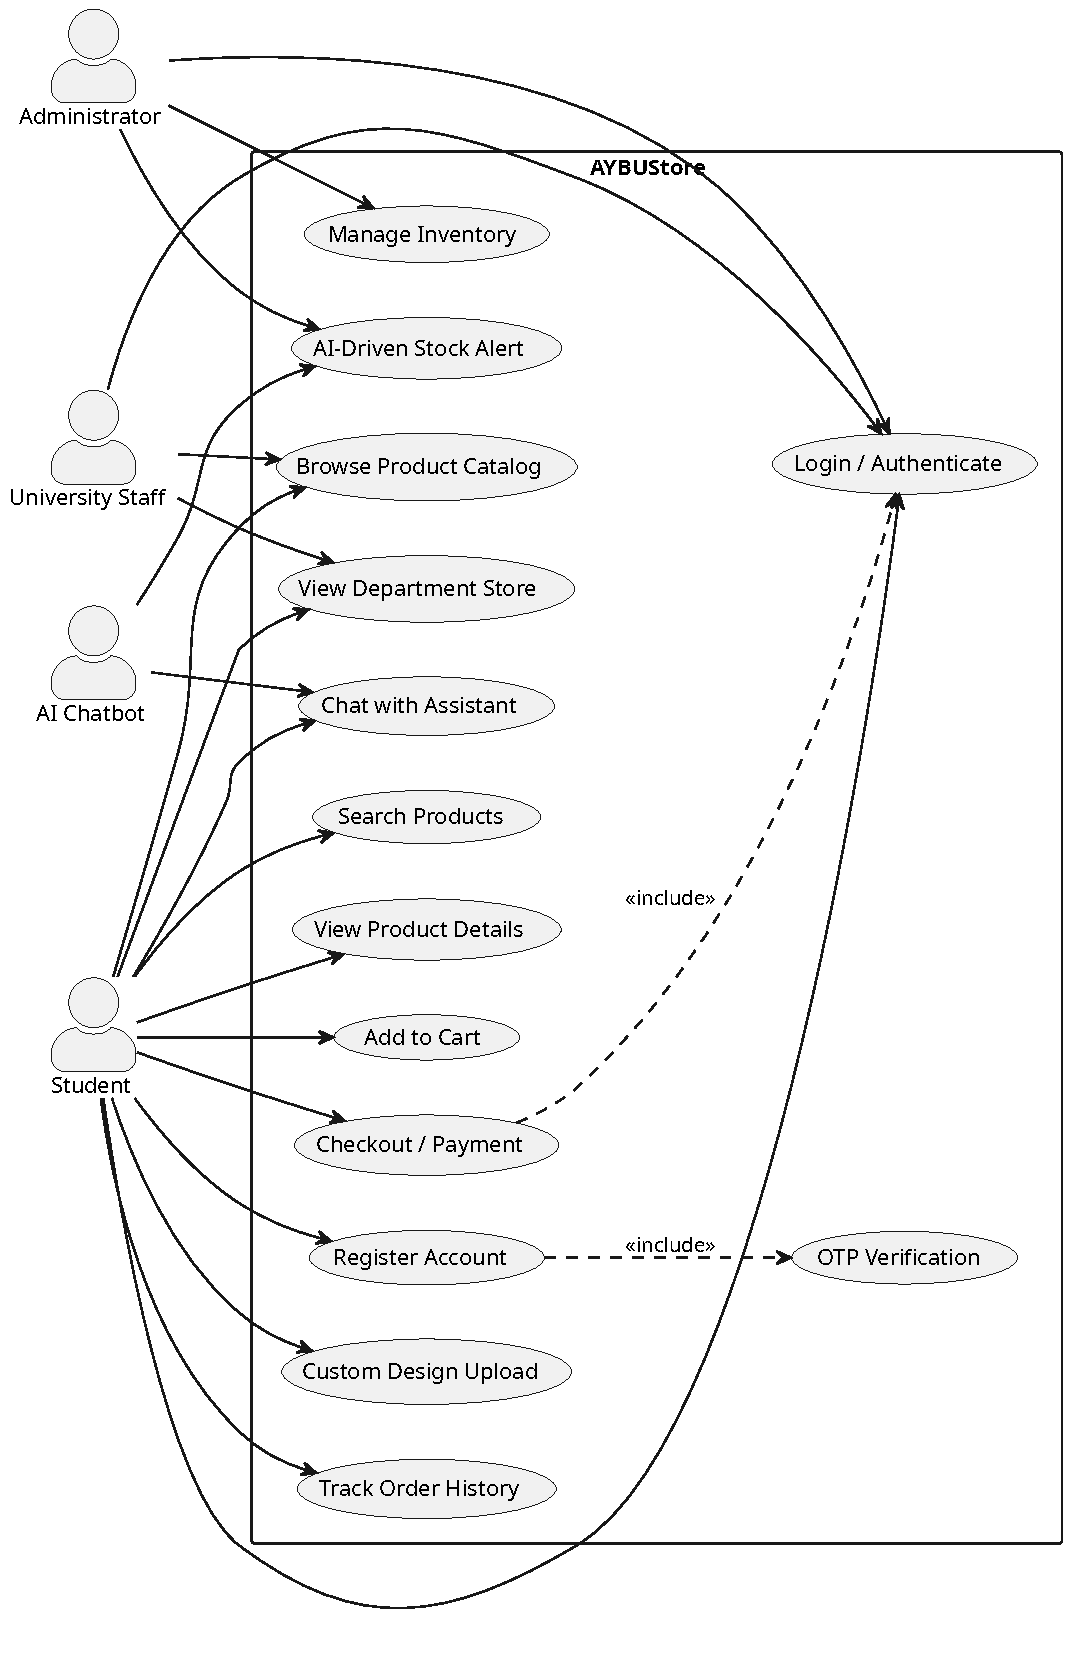
\includegraphics[width=0.96\linewidth,height=0.82\textheight,keepaspectratio]{use_case_diagram.pdf}
    \captionof{figure}{AYBUStore Enterprise Use Case Diagram (Revised)}
\end{center}
\end{landscape}
\clearpage
 
The use case model is organized into five top-level use case groups, each decomposed into more specific sub-use-cases through \texttt{<<include>>} and \texttt{<<extend>>} relationships.
 
\noindent\textbf{Primary Actors:} Student/Staff (the main customer of the platform), Admin (AYBU Staff managing the backoffice), Logistics Coordinator (responsible for routing and dispatch).
 
\noindent\textbf{Secondary Actors (supporting systems):} SIS/OTP Service (handles identity verification), Notification Service (delivers alerts via email and push), AI Engine (provides intent analysis and recommendations).
 
\noindent\textbf{Main Use Cases:}
\begin{enumerate}
    \item \textbf{UC-01 User Access Management} --- groups identity-related flows.
    \begin{itemize}
        \item UC-01.1 Register / Login \texttt{<<include>>} UC-01.2 Verify OTP (mandatory step).
    \end{itemize}
    \item \textbf{UC-02 Product Discovery} --- groups all product-finding flows.
    \begin{itemize}
        \item UC-02.1 Search Catalog (standard filtering).
        \item UC-02.2 AI Recommendations \texttt{<<extend>>} Search Catalog (optional AI-enriched results).
        \item UC-02.3 Customize Merchandise (e.g., personalized hoodie design).
    \end{itemize}
    \item \textbf{UC-03 Order Fulfillment} --- groups the purchase pipeline.
    \begin{itemize}
        \item UC-03.1 Manage Cart \texttt{<<include>>} UC-03.2 Checkout \& Payment \texttt{<<include>>} UC-03.3 Campus Route Planning.
    \end{itemize}
    \item \textbf{UC-04 Tracking \& Support} --- groups post-purchase user interactions.
    \begin{itemize}
        \item UC-04.1 Real-time Tracking.
        \item UC-04.2 Ticket / AI Support \texttt{<<extend>>} Real-time Tracking (triggered when an issue is detected).
    \end{itemize}
    \item \textbf{UC-05 Backoffice Operations} --- groups admin-only flows.
    \begin{itemize}
        \item UC-05.1 Inventory \& Catalog management.
        \item UC-05.2 Order \& Rule Administration.
    \end{itemize}
\end{enumerate}
 
This grouping covers the six-use-case minimum (five top-level groups expanding to thirteen leaf use cases in total) and explicitly models actor responsibilities so that secondary services (SIS/OTP, Notification, AI Engine) remain decoupled from the primary user-facing flows.
 
\subsection{User Stories}
\begin{enumerate}
    \item As a student in Esenboğa, I want to design and order my own hoodie online so that I can avoid traveling to the central campus store.
    \item As an Admin, I want to update stock levels in real time so that users do not place orders for unavailable items.
    \item As a user, I want an AI assistant that understands natural language so that I can find products without knowing exact category names.
    \item As a first-time visitor, I want a secure OTP-based login so that my personal and cart data remain protected.
    \item As a customer, I want real-time order tracking across campuses so that I know exactly when and where my order will arrive.
    \item As a student with a delivery problem, I want a chatbot that resolves common issues instantly so that I do not wait in a queue for trivial questions.
    \item As an Admin, I want an audit log of order and stock changes so that I can investigate disputes and ensure accountability.
\end{enumerate}
 
% ============================================================
% SECTION 7: SYSTEM DESIGN & ARCHITECTURE
% ============================================================
\section{System Design \& Architecture}
\label{sec:system-design}
 
\subsection{Architectural Pattern Selection and Justification}
AYBUStore adopts a \textbf{Layered (n-tier) Architecture with a Serverless Backend}, structured into four logical tiers: (1) the \textit{Presentation Layer} (Next.js + React UI), (2) the \textit{Application Layer} (route handlers and business logic in serverless functions), (3) the \textit{Domain/Service Layer} (Auth, Cart, Order, Logistics, and AI-Assistant services), and (4) the \textit{Data Layer} (Firestore collections and Cloud Storage).
 
This pattern was chosen over alternatives for three reasons. First, compared to a full \textit{microservices} architecture, a layered serverless design avoids the operational overhead (service discovery, distributed tracing, container orchestration) that a five-person student team cannot reasonably sustain during a 14-week schedule. Second, compared to a classical \textit{client-server monolith}, the layered serverless approach gives us elastic auto-scaling and pay-per-use cost characteristics, which directly support NFR-02 (scalability) and the multi-campus traffic distribution requirement. Third, layered separation matches the team's WBS: each work package maps cleanly to one or two layers, enabling parallel development and isolated testing. \textit{MVC} is applied internally within the Presentation Layer (Next.js pages as Controllers, React components as Views, Firestore-backed stores as Models), but it is not sufficient as a top-level architectural pattern because it does not describe the backend service boundaries.
 
\subsection{UML Class Diagram}
\begin{center}
    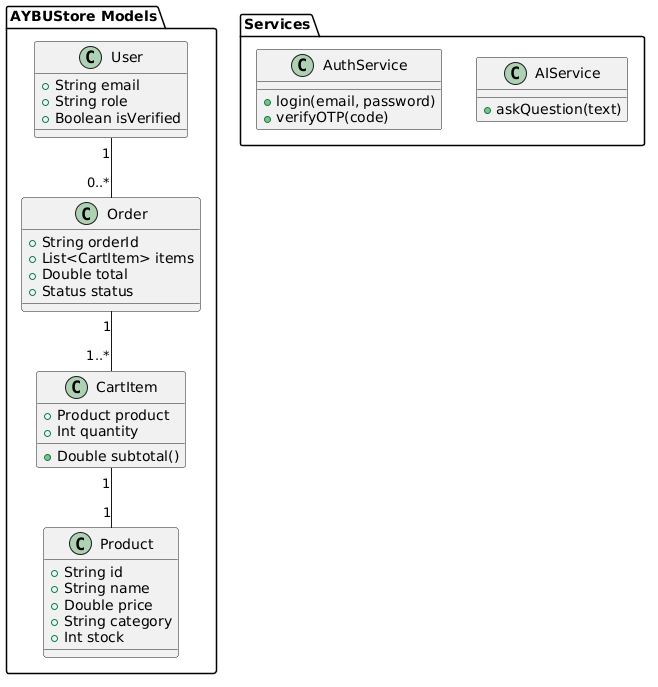
\includegraphics[width=0.9\textwidth]{class_diagram.png}
    \captionof{figure}{System Domain Class Diagram (8 Classes)}
\end{center}
 
The domain model is divided into two contexts (Domain and Operational) and comprises eight classes that satisfy the SRS in Section~\ref{sec:srs}. Each class lists its key attributes and methods.
 
\begin{itemize}
    \item \textbf{User} --- \texttt{uid, email, name, campus, isVerified, role}; \texttt{authenticate(), verifyOTP(code)}. Represents a registered student/staff member, linked to a single Cart and many Orders.
    \item \textbf{Product} --- \texttt{productId, name, category, price, stock, images}; \texttt{updateStock(qty), isAvailable()}. The merchandise unit shown in the catalog.
    \item \textbf{Cart} --- \texttt{cartId, ownerUid, items, total}; \texttt{addItem(p, qty), removeItem(p), recalculate(), checkout()}. Persistent shopping cart owned by exactly one user.
    \item \textbf{Order} --- \texttt{orderId, userId, items, status, campus, createdAt}; \texttt{place(), updateStatus(s), processLogistics()}. The transactional record produced at checkout.
    \item \textbf{Payment} (simulated) --- \texttt{paymentId, orderId, amount, status}; \texttt{authorize(), capture()}. One-to-one with Order; covers the simulated payment lifecycle.
    \item \textbf{LogisticsEngine} --- \texttt{routeId, originCampus, destinationCampus, eta}; \texttt{calculateRoute(order), triggerNotification(uid, msg), assignCourier()}. Computes campus-specific delivery routes (Strategy pattern target).
    \item \textbf{AIAssistant} --- \texttt{sessionId, context}; \texttt{analyzeIntent(query), recommendProduct(user)}. Provides natural-language search and recommendation services.
    \item \textbf{CMSManager} --- \texttt{adminId}; \texttt{updateStock(p, qty), manageCampaign(c), auditLog(action)}. Administrative facade for backoffice operations.
\end{itemize}
 
\noindent\textbf{Key Relationships:}
\begin{itemize}
    \item User \textit{owns} (1:1) Cart; User \textit{places} (1:0..*) Order.
    \item Cart \textit{contains} (1:0..*) Product; Order \textit{includes} (1:1..*) Product.
    \item Order \textit{has} (1:1) Payment; Order is \textit{processedBy} (1:1) LogisticsEngine.
    \item AIAssistant \textit{recommends} Product (dependency); CMSManager \textit{manages} Product and \textit{administers} Order (dependency).
    \item LogisticsEngine \textit{notifies} User (dependency).
\end{itemize}
 
\subsection{UML Sequence Diagrams}
Two key scenarios are modeled with sequence diagrams: user authentication (Scenario 1) and order placement with logistics dispatch (Scenario 2).
 
\noindent\textbf{Scenario 1: Registration and OTP Verification.} The user fills the registration form rendered by the \texttt{StorefrontAuth} React component. Each keystroke triggers \texttt{updateAuthField(field, value)} on the \texttt{useAuthForm} hook, which maintains and validates the local form state. On submission, \texttt{handleAuthSubmit("register")} is invoked: the hook first runs \texttt{isAuthSubmittable()} to gate the request, then sets the submit status to ``loading'' and calls \texttt{createUserWithEmailAndPassword} on the Firebase Auth SDK. Firebase Cloud persists the user record and returns a \texttt{UserCredential}; the hook then calls \texttt{updateProfile(displayName)}. Upon success, the status flips to ``otp'' and the UI renders the 6-digit OTP input screen. The user enters the code, the hook calls \texttt{verifyOTP(code)}, and on confirmation the status becomes ``success'', redirecting the user to the dashboard.
 
\begin{center}
    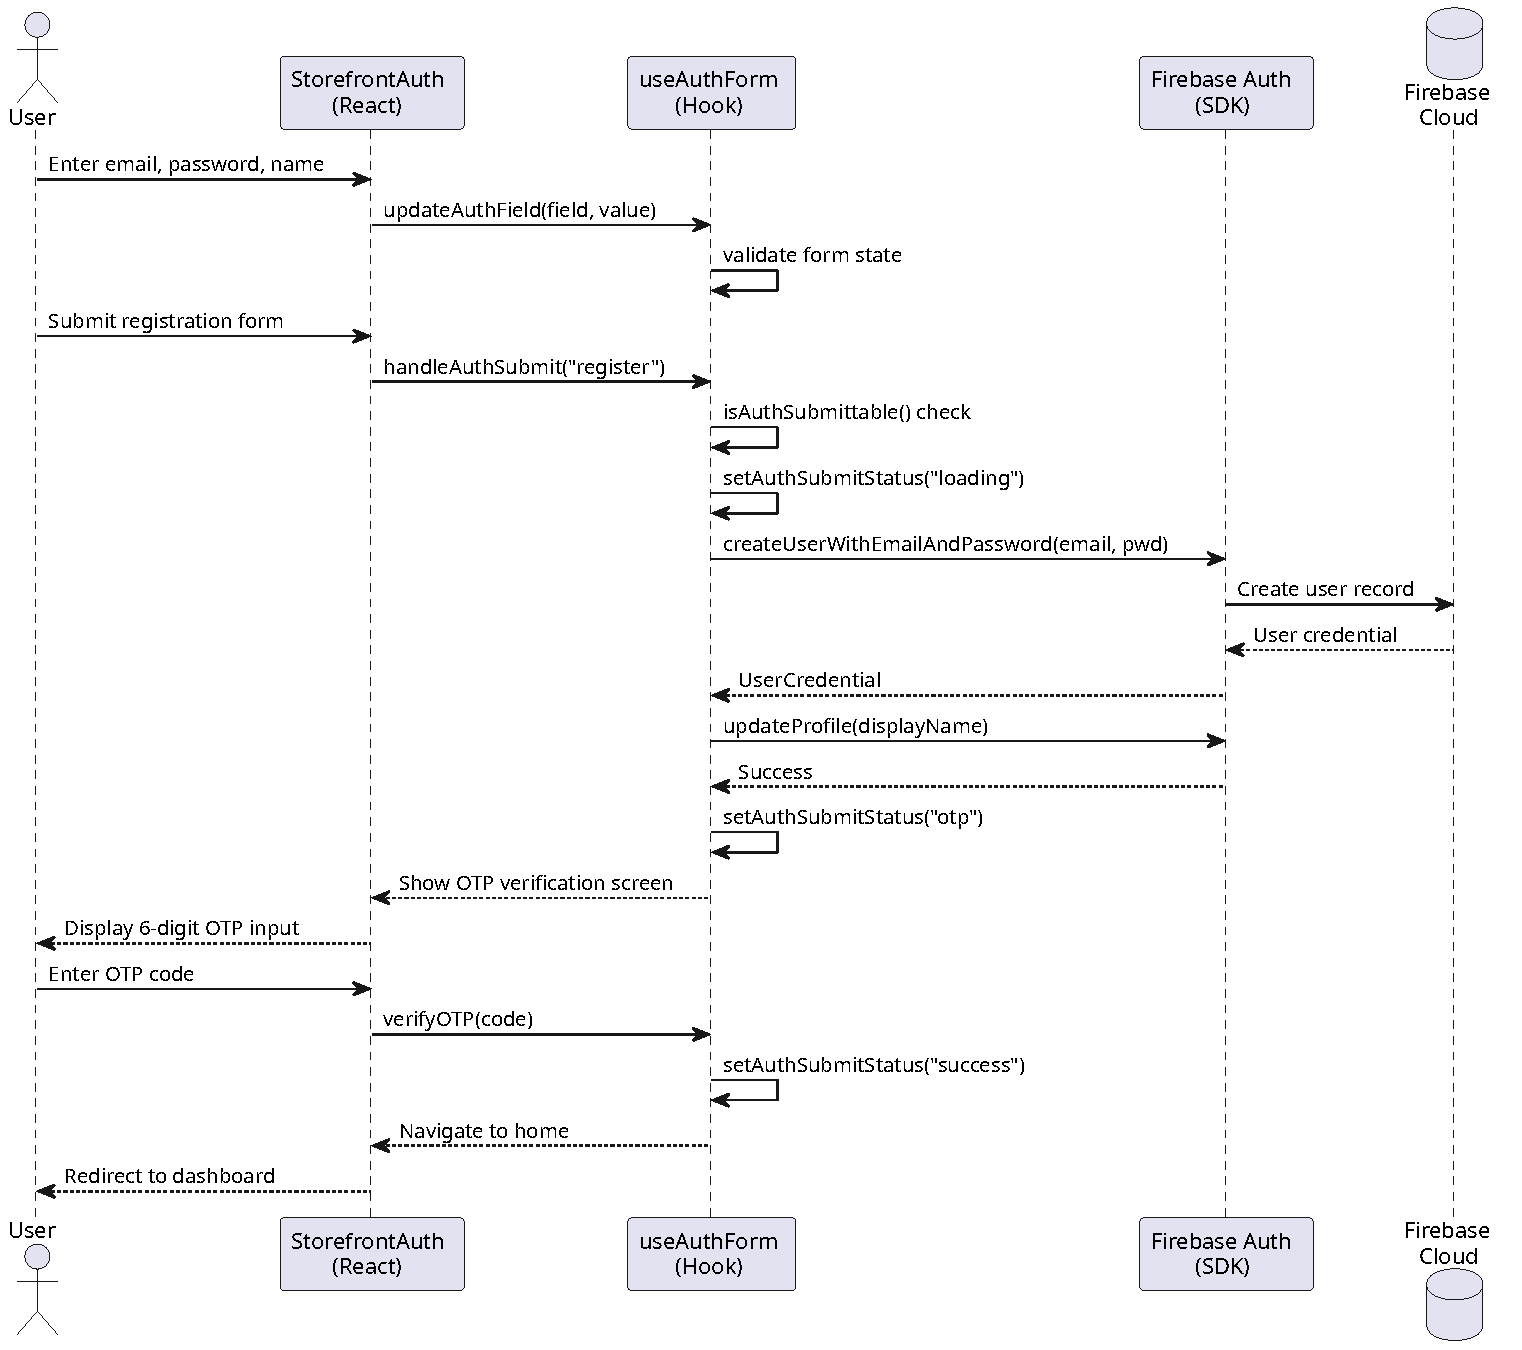
\includegraphics[width=0.8\textwidth]{sequence_auth.pdf}
    \captionof{figure}{Scenario 1: Registration and OTP Verification}
\end{center}
 
\noindent\textbf{Scenario 2: Order Placement and Logistics Dispatch.} The user clicks ``Place Order'' on the Next.js UI, which calls \texttt{submitOrder(cart, campus)} on the Order Service. The Order Service first calls \texttt{checkStock(items[])} on the Product Service, which reads stock from Firestore and returns \texttt{stockOK = true}. The Order Service then opens a Firestore transaction (\texttt{BEGIN transaction}), decrements stock, inserts the order with \texttt{status="Placed"}, and receives the generated \texttt{orderId}. It then calls \texttt{authorize(amount)} on the simulated Payment Service; on \texttt{paymentOK}, the transaction is committed. The Order Service next calls \texttt{dispatch(orderId, campus)} on the Logistics Service, which uses the Strategy pattern to select the campus-specific routing strategy, inserts the route into Firestore, assigns a courier, and replies with \texttt{routeAssigned}. The Order Service then invokes \texttt{sendConfirmation(userId, orderId)} on the Notification Service, which emails and pushes an in-app notification to the user. Finally, the Order Service replies with \texttt{orderConfirmation(orderId, eta)} and the UI shows the summary and tracking link.
 
\begin{center}
    \includegraphics[width=0.85\textwidth]{sequence_order.png}
    \captionof{figure}{Scenario 2: Order Placement and Logistics Dispatch}
\end{center}
 
\subsection{UML Activity Diagram}
\begin{center}
    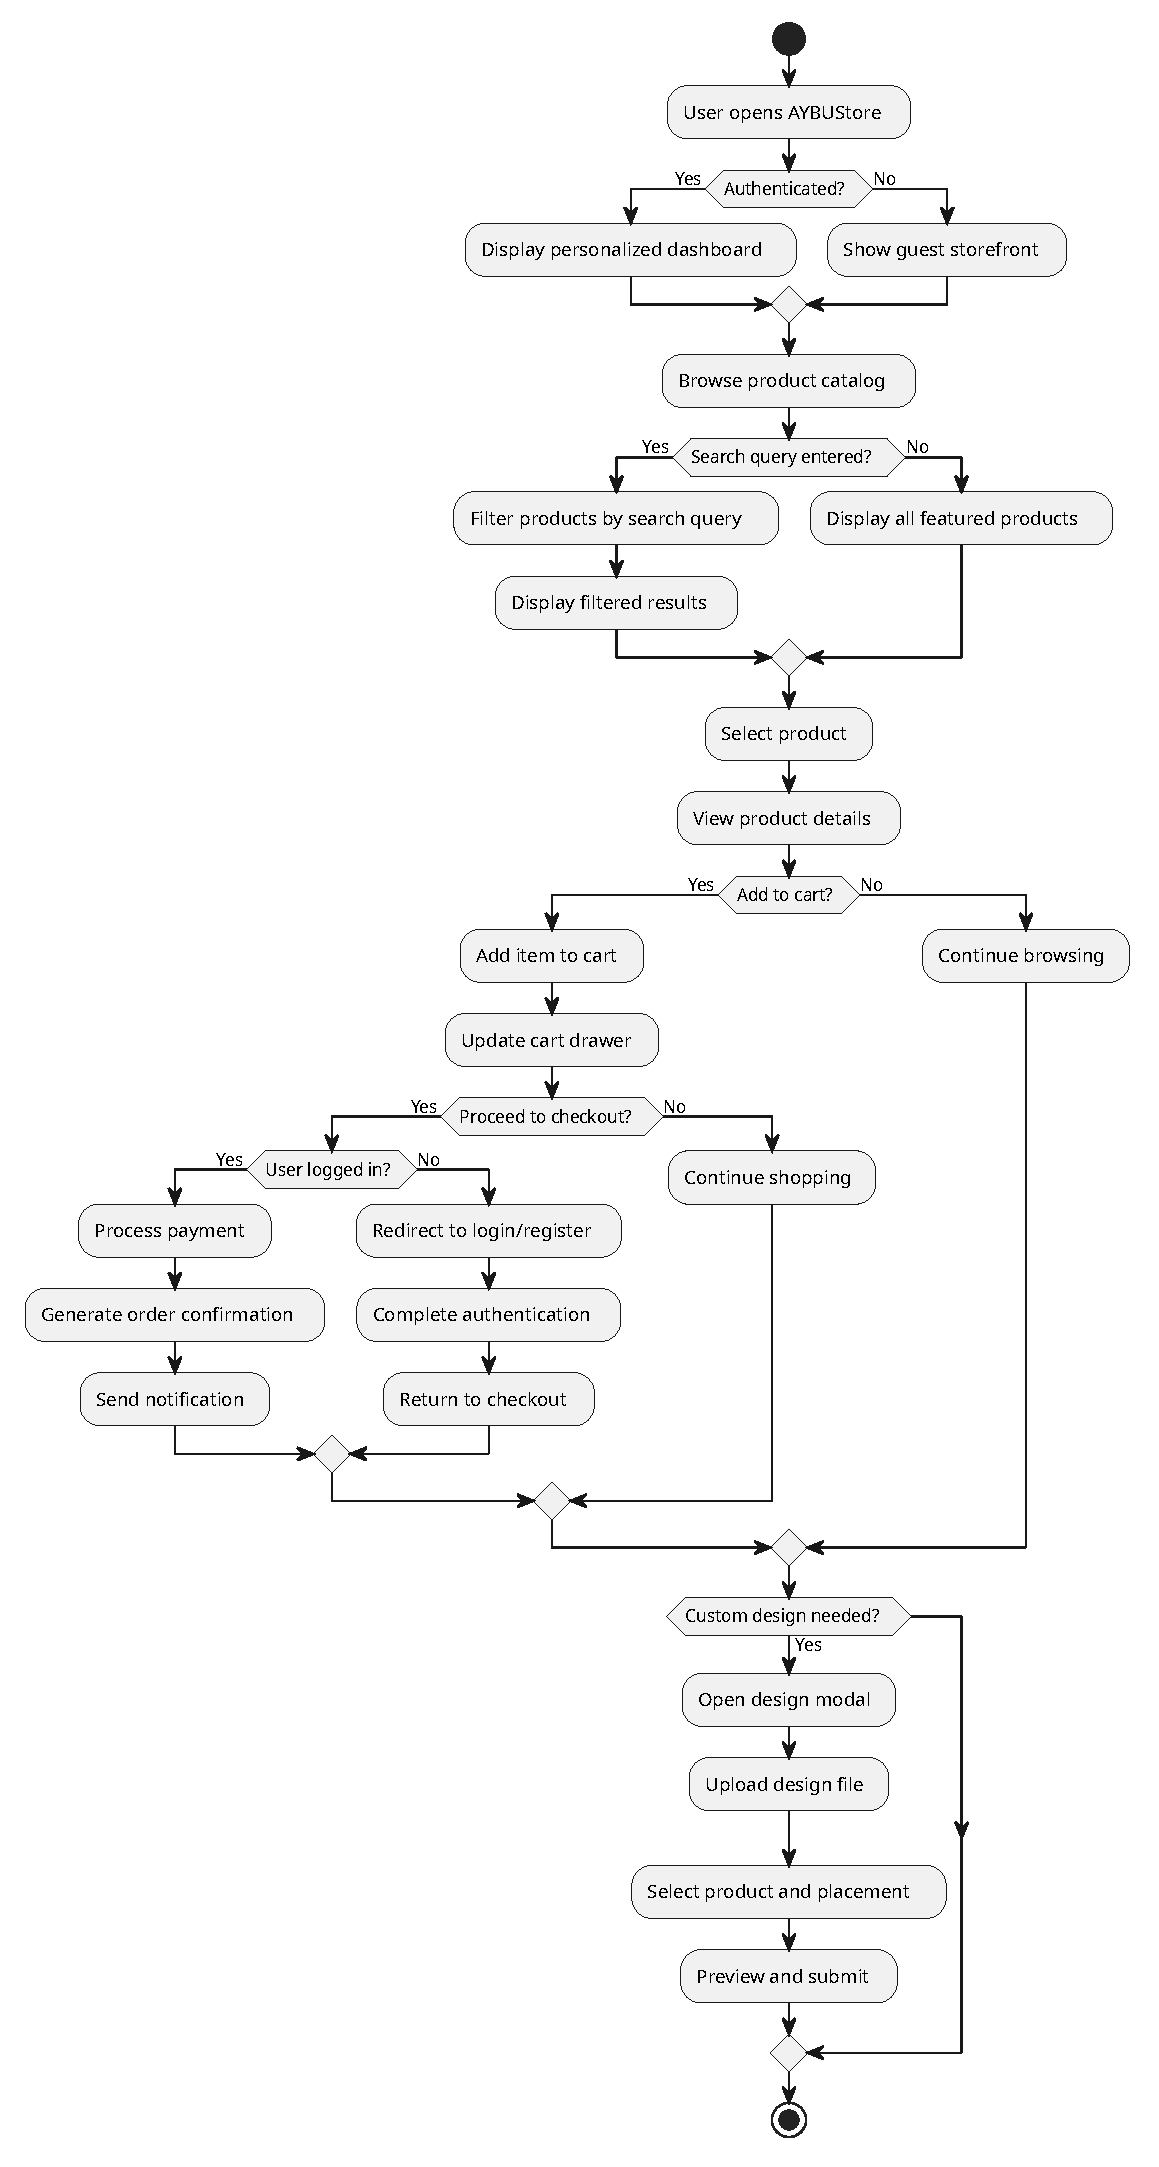
\includegraphics[width=0.8\textwidth]{activity_diagram.pdf}
    \captionof{figure}{Phase 4: Logistics and Notification Pipeline}
\end{center}
 
The activity diagram models the Phase~4 pipeline that fires after a user confirms an order. The flow proceeds through three stages. (1) \textit{Intent and Routing}: the AI layer briefly performs intent analysis on the order context, then the system determines the user's campus location. A decision node branches on ``Esenboğa Campus?'': if \textit{yes}, the order is routed to the Central Warehouse; if \textit{no}, it is routed to the appropriate Local Satellite Hub (Etlik, Bilkent, or Çubuk). (2) \textit{Inventory Sync}: regardless of branch, the Firestore inventory is updated to reflect the assignment. (3) \textit{Notification Pipeline}: a Firebase Cloud Function is triggered, which generates a logistics token, dispatches a real-time push notification, and updates the user's tracking UI. The end state is a tracked, observable order visible in the user's dashboard.
 
\subsection{GoF Design Patterns}
Three Gang-of-Four patterns are applied:
 
\begin{enumerate}
    \item \textbf{Singleton (Creational)} --- Used for the Firebase service instance and the AI-Assistant context manager. \textit{Justification:} multiple SDK initializations would create connection leaks and inconsistent auth state; a single managed instance per runtime guarantees correctness.
    \item \textbf{Strategy (Behavioral)} --- Used for campus-specific logistics routing. Each campus (Esenboğa, Etlik, Bilkent, Çubuk) has a distinct routing rule and ETA computation. \textit{Justification:} the \texttt{LogisticsEngine} class can swap strategies at runtime without modifying the Order Service, satisfying the Open/Closed principle (see SOLID below).
    \item \textbf{Observer (Behavioral)} --- Used for cart state synchronization across UI components and for real-time order tracking via Firestore listeners. \textit{Justification:} multiple subscribers (cart icon, checkout page, admin dashboard) must react to the same state change without tight coupling to the source.
\end{enumerate}
 
A fourth pattern, \textbf{Factory Method}, is also used internally by the Notification Service to instantiate the correct channel handler (email vs. in-app), keeping notification dispatch extensible.
 
\subsection{SOLID Principles Applied}
\begin{itemize}
    \item \textbf{Single Responsibility:} Each service class (Auth, Cart, Order, Logistics, Notification) owns exactly one domain concern; UI components do not contain business logic.
    \item \textbf{Open/Closed:} New logistics strategies (e.g., adding a fifth campus or an off-peak routing variant) are added by creating a new Strategy class, not by modifying \texttt{LogisticsEngine}.
    \item \textbf{Liskov Substitution:} Notification channel classes (\texttt{EmailNotifier}, \texttt{InAppNotifier}) are interchangeable through the \texttt{Notifier} interface; callers depend only on the contract.
    \item \textbf{Interface Segregation:} Admin and customer APIs are separated; customer-facing components never expose admin-only methods, reducing accidental privilege escalation.
    \item \textbf{Dependency Inversion:} High-level services (Order, Cart) depend on abstractions (\texttt{IRepository}, \texttt{INotifier}) rather than on Firestore SDK calls directly; this decouples the frontend from any specific backend implementation and allows mocking during unit tests.
\end{itemize}
 
\subsection{Quality Attribute Trade-offs}
Architectural decisions involve explicit trade-offs:
 
\begin{itemize}
    \item \textbf{Performance vs.\ Security:} Aggressive edge caching (CDN, ISR in Next.js) reduces TTI but risks serving stale data for stock and order status. We resolve this by caching only catalog data with short TTLs and serving authenticated, stock-sensitive views via server-rendered, non-cached routes. Authentication endpoints bypass caching entirely.
    \item \textbf{Scalability vs.\ Simplicity:} A microservices design would scale services independently, but introduces operational complexity disproportionate to a student-team pilot. The serverless layered approach gives sufficient elasticity (Firebase Functions auto-scale per request) while keeping the codebase small enough for the team to reason about as a whole.
    \item \textbf{Consistency vs.\ Availability:} Firestore offers strong consistency within a document and eventual consistency across listeners. Order placement uses transactions for stock decrement (favoring consistency), while non-critical UI updates (recommendation feed, badge counters) tolerate eventual consistency for higher availability.
    \item \textbf{Cost vs.\ Reliability:} Pay-per-invocation pricing keeps idle cost near zero, but bursty traffic can spike costs. We mitigate with per-user request quotas and admin-side rate limits, accepting that extreme traffic spikes (e.g., flash campaigns) may degrade gracefully rather than scale without bound.
    \item \textbf{Usability vs.\ Security:} OTP verification adds a friction step at login. We accept this trade-off because NFR-04 (security) and the institutional-data context (SIS-linked accounts) make unauthenticated or weakly authenticated access unacceptable. Session lifetimes are tuned long enough that returning users rarely re-verify.
\end{itemize}
 
\newpage
 
 
% ============================================================
% SECTION 8: TEAM & RESOURCE PLAN
% ============================================================
\section{Team \& Resource Plan}
\label{sec:team-resource-plan}
 
AYBUStore will be developed by a five-member student team during the
14--15 week academic project period. The project combines a campus-focused
digital storefront, secure OTP authentication, Firebase-based backend
services, product catalogue management, cart and simulated checkout flows,
admin/CMS operations, campus-aware order tracking, rule-based support
assistance, testing, and documentation. Therefore, team responsibilities
are distributed according to the main software engineering activities and
system modules. This role distribution supports the Agile/Scrum process
defined in the methodology section and ensures that each major component
has a clear owner.
 
\subsection{Team Members, Roles, and Responsibilities}
 
\renewcommand{\arraystretch}{1.25}
\begin{table}[H]
\centering
\small
\begin{tabularx}{\textwidth}{|p{0.20\textwidth}|p{0.24\textwidth}|X|}
\hline
\rowcolor{aybuHeader}
\textcolor{white}{\textbf{Team Member}} &
\textcolor{white}{\textbf{Role}} &
\textcolor{white}{\textbf{Responsibilities}} \\ \hline
 
Muhammed Yıldız &
Project Manager / Product Owner &
Coordinates the overall project schedule, manages the product backlog,
communicates with stakeholders, monitors sprint progress, and checks the
consistency between requirements, design, implementation plan, and
evaluation criteria. \\ \hline
 
Utkan Dindaroğlu &
Frontend Developer / UI-UX Designer &
Designs and develops the responsive web client and mobile-oriented user
interface. Responsible for catalogue browsing, product detail pages, cart
views, simulated checkout screens, and usability improvements across web
and mobile views. \\ \hline
 
Ahmet Selim Yılmaz &
Backend Developer / Database Engineer &
Manages Firebase-based backend services and Firestore database structure.
Responsible for user accounts, product catalogue data, categories, carts,
orders, inventory records, support tickets, and related data management. \\ \hline
 
Seyfullah Gülyazı &
Evaluation and Resource Planning Responsible / QA Support &
Prepares the Team and Resource Plan, Expected Outcomes, and Evaluation
Plan sections. Supports acceptance test planning, success criteria
definition, cost estimation consistency, and final documentation quality
control. \\ \hline
 
Süleyman Fatih Sert &
Tracking, Support, and Admin Module Developer &
Contributes to OTP/authentication flows, admin/CMS operations, inventory
management, order status operations, campus-aware tracking, rule-based
support logic, and testing of critical customer and administrator workflows. \\ \hline
 
\end{tabularx}
\caption{Team members, roles, and responsibilities for AYBUStore.}
\label{tab:team-roles}
\end{table}
 
\subsection{Hardware Resources}
 
No special-purpose hardware is required for AYBUStore. The personal laptops
of the team members are sufficient for development, testing, documentation,
and presentation preparation. A stable internet connection is required for
GitHub collaboration, Firebase access, cloud deployment, online meetings,
and shared documentation work. Mobile devices or browser-based emulators
will be used to check the responsive behaviour of the application, while
standard browsers such as Chrome, Edge, and Firefox will be used for
cross-browser testing. Since all required hardware resources are already
available to the team, no additional hardware cost is expected during the
academic prototype and documentation stage.
 
\subsection{Software Resources}
 
The project will use commonly available software engineering and web
development tools. Visual Studio Code will be used as the main development
environment, while Git and GitHub will be used for version control and
collaborative development. A responsive web client structure will support
cross-platform access, and Firebase services will be used for authentication,
backend logic, and database management. Firestore will store user accounts,
product catalogue data, categories, cart records, orders, inventory
information, support tickets, and tracking-related data. Draw.io, Lucidchart,
or PlantUML will be used for UML diagrams, while Figma may be used for UI/UX
mockups. Postman, Firebase Console, and browser developer tools will support
testing and debugging. Microsoft Word, Google Docs, PowerPoint, or Google
Slides will be used for documentation and final presentation preparation.
 
\subsection{Cloud and API Resources}
 
AYBUStore is planned as a low-cost cloud-supported academic project. Firebase
Authentication will be used for secure OTP-based user authentication, and
Firebase Firestore will be used as the main cloud database. Firebase Cloud
Functions may be used for backend operations such as stock deduction, order
state updates, campus-routing logic, notification-related logic, and support
workflow operations. Firebase Storage may be used for product images, while
Firebase Hosting or a similar hosting service may be used if a web prototype
is deployed.
 
Payment operations are treated as simulated in the current project phase, so
no live third-party payment transaction cost is expected. Firebase Security
Rules will be used to protect user, product, order, support, and administrator
data. Live integration with AYBU internal SIS/ERP systems, off-campus delivery
operations, GPS-based physical logistics tracking, and advanced predictive
AI/ML features such as deep personalization or demand forecasting are outside
the current project scope. Only rule-based automated support and simple
product-search assistance are considered within the prototype-level support
logic.
 
\subsection{Estimated Project Cost}
 
Since AYBUStore is an academic course project, no actual salary will be paid
to the team members. However, a notional project cost is estimated to show the
commercial value of the required effort and infrastructure. This estimation
is kept consistent with the COCOMO-based effort and cost estimation used in
the Methodology and Development Plan section.
 
According to the COCOMO-based estimation, the project requires approximately
17.2 person-months of effort. If a junior developer cost of \$1{,}500 per
person-month is assumed, the notional labour cost is calculated as follows:
 
\[
17.2 \text{ person-months} \times 1500 \text{ USD/person-month}
= 25{,}800 \text{ USD}
\]
 
Most development tools and cloud services will be used through free-tier or
academic-accessible plans. Therefore, only a small infrastructure buffer is
included for possible Firebase or hosting overages during testing.
 
\renewcommand{\arraystretch}{1.25}
\begin{table}[H]
\centering
\small
\begin{tabularx}{0.88\textwidth}{|X|r|}
\hline
\rowcolor{aybuHeader}
\textcolor{white}{\textbf{Resource / Cost Item}} &
\textcolor{white}{\textbf{Estimated Cost}} \\ \hline
 
Personal computers and internet access & 0 USD \\ \hline
GitHub, Visual Studio Code, Draw.io / PlantUML & 0 USD \\ \hline
Figma Free Plan or academic-accessible design tools & 0 USD \\ \hline
Firebase Free Tier / minor development overages & 100 USD \\ \hline
Firebase Hosting or similar hosting service & 0 USD \\ \hline
Simulated payment flow / test-mode tooling & 0 USD \\ \hline
Notional labour cost & 25{,}800 USD \\ \hline
\textbf{Total estimated project cost} & \textbf{25{,}900 USD} \\ \hline
 
\end{tabularx}
\caption{Estimated team and infrastructure cost for AYBUStore.}
\label{tab:team-resource-cost}
\end{table}
 
The actual out-of-pocket cost is expected to remain very low because the
project mainly uses free-tier tools, academic-accessible services, and
simulated/test-mode integrations. When the notional labour effort and the
small infrastructure buffer are included, the total estimated project cost
becomes approximately 25{,}900 USD.
 
 
% ============================================================
% SECTION 9: EXPECTED OUTCOMES & EVALUATION PLAN
% ============================================================
\section{Expected Outcomes \& Evaluation Plan}
\label{sec:expected-outcomes-evaluation}
 
The AYBUStore project is expected to produce a reference-level
prototype and a complete software engineering documentation package
for a campus-focused digital commerce ecosystem. The evaluation plan
is designed to verify whether the system supports the main user,
administrator, and operational workflows defined in the project scope.
It also checks whether the project meets its measurable targets related
to cross-campus access, OTP-based security, platform responsiveness,
support efficiency, and operational reliability.
 
\subsection{Expected Artefacts}
 
The following artefacts are expected to be produced at the end of the
project:
 
\begin{itemize}[leftmargin=*]
    \item \textbf{AYBUStore reference prototype:} A campus-focused
    digital storefront demonstrating product search, cart operations,
    simulated checkout, order creation, and order tracking flows.
 
    \item \textbf{OTP-based authentication module:} A secure
    registration and login flow for protected user and order-related
    actions.
 
    \item \textbf{Product catalogue and search module:} A module for
    listing AYBU-specific products, searching products by keywords, and
    displaying product details.
 
    \item \textbf{Cart and simulated checkout module:} A structure that
    allows users to add products to the cart and complete the order flow
    without live third-party payment processing.
 
    \item \textbf{Campus-aware order tracking module:} A tracking
    structure that displays order status information for Esenboga,
    Etlik, Bilkent, and Cubuk campuses.
 
    \item \textbf{Rule-based AI support layer:} A simple support and
    product-discovery layer for first-level user assistance based on
    predefined rules and intent patterns.
 
    \item \textbf{Admin/CMS and inventory module:} An administrator
    panel for managing products, stock information, orders, and
    operational data.
 
    \item \textbf{Software engineering documentation:} SRS, UML
    diagrams, architectural design, WBS, Gantt chart, risk management
    table, test plan, final report, and presentation slides.
\end{itemize}
 
\subsection{Success Measurement}
 
The project will be considered successful if the following conditions
are satisfied:
 
\begin{itemize}[leftmargin=*]
    \item Users can complete the main workflow: authentication, product
    search, cart operation, simulated checkout, and order tracking.
 
    \item OTP-based authentication works correctly and prevents
    unauthorized access to protected user and order data.
 
    \item The system supports AYBU's four-campus structure and displays
    campus-related order status information correctly.
 
    \item The pilot evaluation reaches at least 300 active
    SIS-verified users and shows at least 30\% improvement in
    cross-campus access utilization compared with the baseline.
 
    \item The main storefront achieves a Time to Interactive value
    below 1.5 seconds or shows at least 40\% improvement compared with
    the baseline value of approximately 3.5 seconds.
 
    \item The support process achieves at least 60\% reduction in first
    response time and at least 45\% reduction in average issue-resolution
    time compared with the baseline.
 
    \item Order, stock, tracking, and notification operations remain
    reliable, with 99.9\% service uptime during the pilot window and
    0\% transaction-level data loss.
 
    \item The final documentation remains internally consistent:
    objectives, scope, requirements, UML diagrams, development plan,
    risks, and test cases must align with each other.
\end{itemize}
 
\subsection{Acceptance Test Plan}
 
The acceptance test plan verifies whether AYBUStore satisfies its main
functional, performance, and operational requirements. The following
five test cases focus on the most important project objectives.
 
\renewcommand{\arraystretch}{1.25}
\begin{table}[H]
\centering
\small
\begin{tabularx}{\textwidth}{|p{0.10\textwidth}|p{0.22\textwidth}|X|X|}
\hline
\rowcolor{aybuHeader}
\textcolor{white}{\textbf{Test ID}} &
\textcolor{white}{\textbf{Test Scenario}} &
\textcolor{white}{\textbf{Test Description}} &
\textcolor{white}{\textbf{Expected Success Criteria}} \\
\hline
 
AT-01 &
OTP Authentication &
A registered user enters a valid OTP code during login or registration. &
The user is authenticated successfully and can access protected
features such as cart, profile, and order tracking. \\
\hline
 
AT-02 &
AI-Assisted Product Search &
A user searches for a product using a phrase such as ``hoodie'' or
``white sweat'', or enters a simple first-level support request. &
The system correctly interprets the user intent and returns relevant
product results or an appropriate rule-based support response. \\
\hline
 
AT-03 &
Cart, Simulated Checkout, and Stock Update &
A user adds a product to the cart, completes the simulated checkout
flow, and creates an order. &
The order is created successfully, appears in the user's order history,
and the related product stock information is updated correctly. \\
\hline
 
AT-04 &
Campus-Aware Order Tracking &
A user opens the tracking page for an existing order. &
The system displays the correct order status and related campus
information for Esenboga, Etlik, Bilkent, or Cubuk. \\
\hline
 
AT-05 &
TTI and Pilot Performance Measurement &
The main storefront is tested under standard pilot network conditions. &
The average Time to Interactive value is below 1.5 seconds or shows at
least 40\% improvement compared with the baseline value of
approximately 3.5 seconds. \\
\hline
 
\end{tabularx}
\caption{Acceptance test plan for AYBUStore.}
\label{tab:acceptance-tests-39}
\end{table}
 
\subsection{Evaluation Summary}
 
The evaluation of AYBUStore will combine functional testing,
acceptance testing, performance measurement, operational KPI tracking,
and documentation consistency checks. Functional testing will verify
authentication, product search, cart operations, simulated checkout,
stock updates, campus-aware tracking, and administrator workflows.
Performance evaluation will focus on the Time to Interactive target,
while operational evaluation will focus on cross-campus access
improvement and support-response efficiency. The project will be
accepted as successful if the core workflows pass the defined
acceptance tests, the measurable pilot targets are satisfied, and the
final documentation remains consistent with the project objectives,
scope, architecture, and development plan.
 
 
\section{Conclusion}
The AYBUStore project represents a successful fusion of modern software engineering methodologies and institutional needs. By collaborating with the \textbf{AYBU IT Department}, we have ensured that the platform is not merely a standalone application, but a robust, secure, and scalable extension of the university's digital brand.
 
Our results demonstrate that hyper-local e-commerce, when augmented with AI-driven personalization and real-time logistics, can significantly enhance merchandise accessibility across geographically distributed campuses. Moving forward, the modular architecture of AYBUStore allows for the integration of further smart-campus features, such as department-specific resource sharing and event-based merchandise launches. Ultimately, this project serves as a technical benchmark for digital transformation within Ankara Yıldırım Beyazıt University, providing a blueprint for future student-centric software solutions.
 
\newpage
\section{References}
\begin{enumerate}[label={[\arabic*]}]
    \item Alenezi, M., Akour, M. 2023. ``Digital transformation blueprint in higher education: A case study of PSU'', \textit{Sustainability}, 15 (10), 8204. DOI: 10.3390/su15108204.
    \item Alsheyadi, A. K., Albalushi, J. 2020. ``Service quality of student services and student satisfaction: The mediating effect of cross-functional collaboration'', \textit{The TQM Journal}. DOI: 10.1108/TQM-10-2019-0234.
    \item Brdesee, H., Alsaggaf, W. 2022. ``Decision-making strategy for digital transformation: A two-year analytical study and follow-up concerning innovative improvements in university e-services'', \textit{Journal of Theoretical and Applied Electronic Commerce Research}, 17 (1), 138--164. DOI: 10.3390/jtaer17010008.
    \item Dinh, H., Tran, T. K. 2023. ``EduChat: An AI-based chatbot for university-related information using a hybrid approach'', \textit{Applied Sciences}, 13 (22), 12446. DOI: 10.3390/app132212446.
    \item Gong, T., Yi, Y. 2018. ``The effect of service quality on customer satisfaction, loyalty, and happiness in five Asian countries'', \textit{Psychology \& Marketing}, 35 (6), 427--442. DOI: 10.1002/mar.21096.
    \item Güldal, H., Dinçer, E. O. 2025. ``Can rule-based educational chatbots be an acceptable alternative for students in higher education?'', \textit{Education and Information Technologies}, 30, 3979--4012. DOI: 10.1007/s10639-024-12977-5.
    \item Jahromi, H. Z., Delaney, D. T., Hines, A. 2020. ``Beyond first impressions: Estimating quality of experience for interactive web applications'', \textit{IEEE Access}, 8, 47741--47755. DOI: 10.1109/ACCESS.2020.2979385.
    \item Liu, D., Deng, Z., Zhang, W., Wang, Y., Kaisar, E. I. 2021. ``Design of sustainable urban electronic grocery distribution network'', \textit{Alexandria Engineering Journal}, 60 (1), 145--157. DOI: 10.1016/j.aej.2020.06.051.
    \item Melkonyan, A., Gruchmann, T., Lohmar, F., Bleischwitz, R., Spinler, S. 2020. ``Sustainability assessment of last-mile logistics and distribution strategies: The case of local food networks'', \textit{International Journal of Production Economics}, 228, 107746. DOI: 10.1016/j.ijpe.2020.107746.
    \item Netravali, R., Nathan, V., Mickens, J., Balakrishnan, H. 2018. ``Vesper: Measuring time-to-interactivity for web pages'', \textit{15th USENIX Symposium on Networked Systems Design and Implementation (NSDI 18)}, 217--231. İnternet adresi: \url{https://www.usenix.org/conference/nsdi18/presentation/netravali-vesper}, Son erişim tarihi: 12 Mayıs 2026.
    \item Suryawanshi, P., Dutta, P., L, V., G, D. 2021. ``Sustainable and resilience planning for the supply chain of online hyperlocal grocery services'', \textit{Sustainable Production and Consumption}, 28, 496--518. DOI: 10.1016/j.spc.2021.05.001.
    \item Urquhart, R., Newing, A., Hood, N., Heppenstall, A. 2022. ``Last-mile capacity constraints in online grocery fulfilment in Great Britain'', \textit{Journal of Theoretical and Applied Electronic Commerce Research}, 17 (2), 636--651. DOI: 10.3390/jtaer17020033.
\end{enumerate}
 
\end{document}
